\chapter{\label{appendix::A}A}
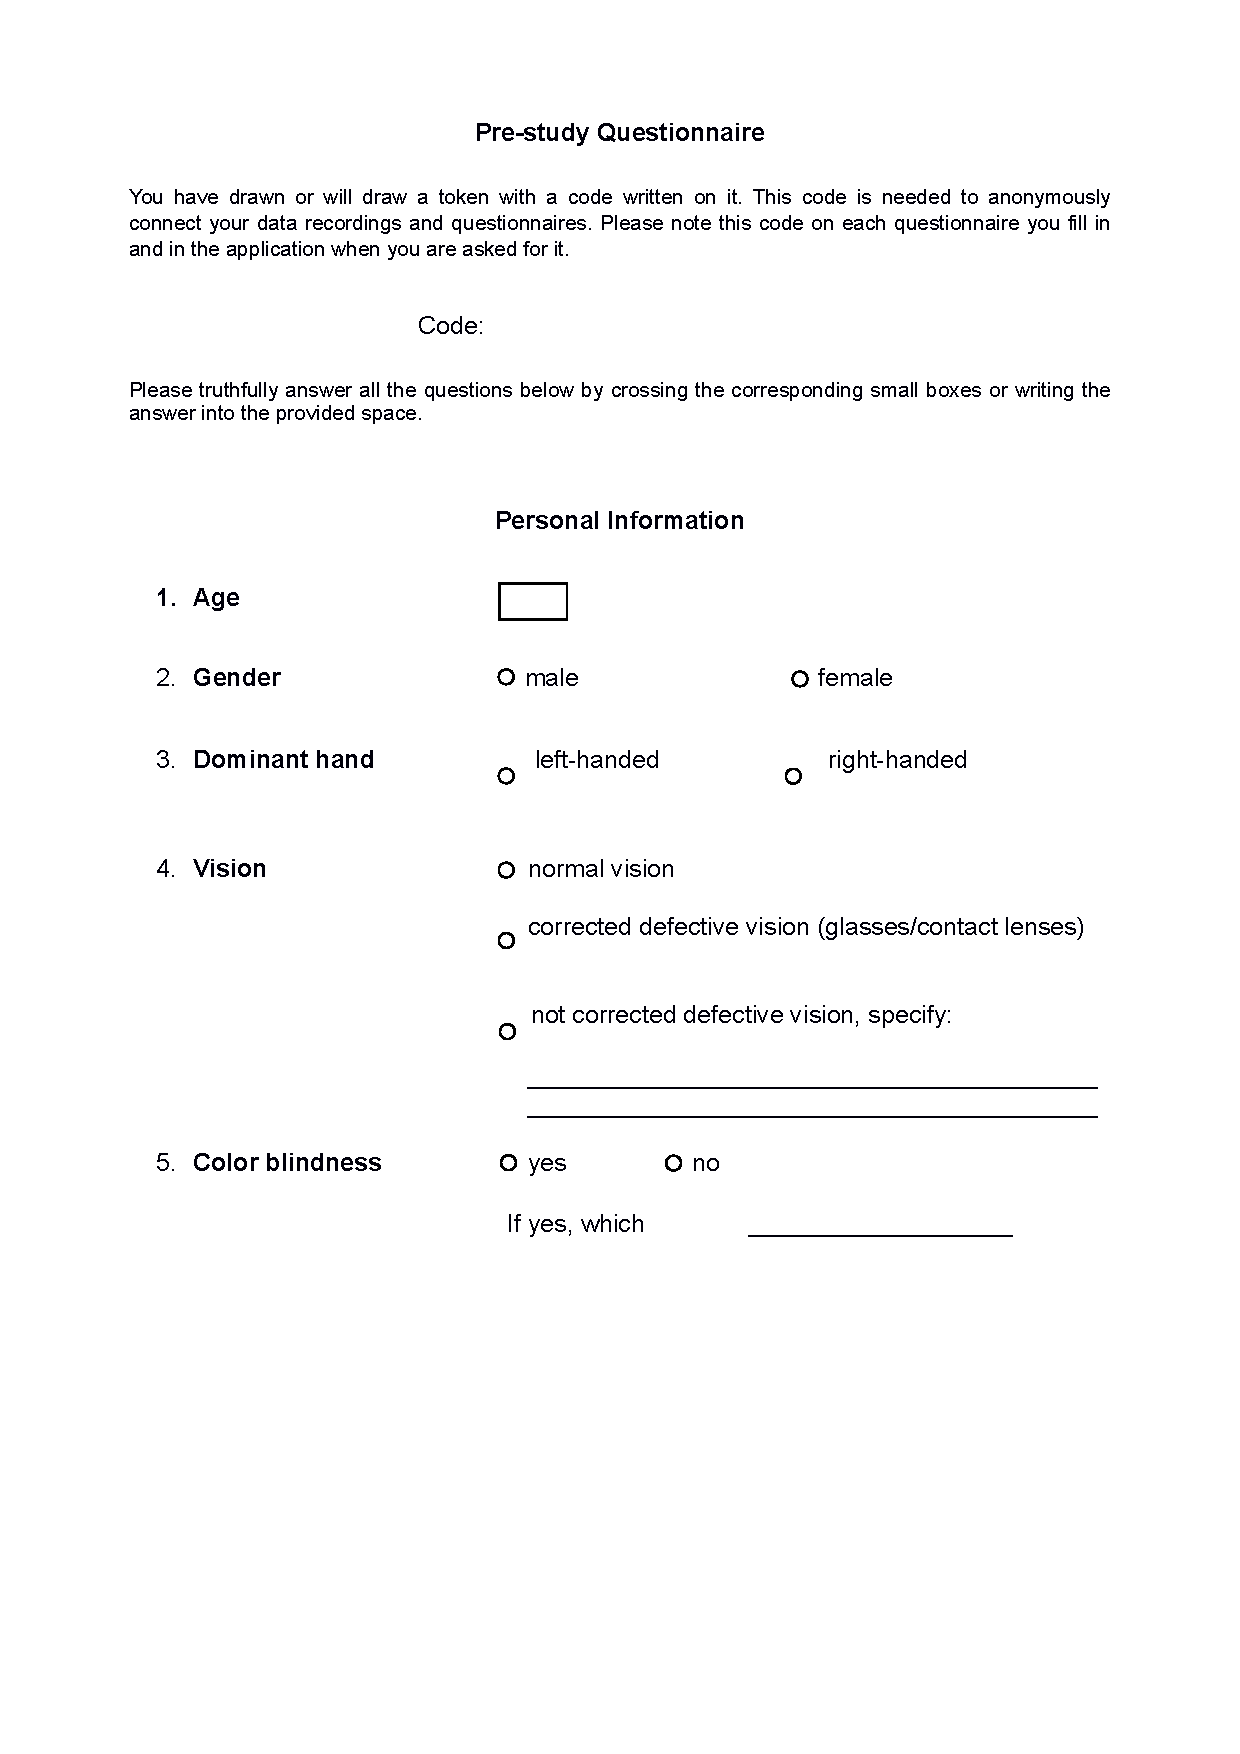
\includepdf[pages=-]{appendix/PreStudy.pdf}
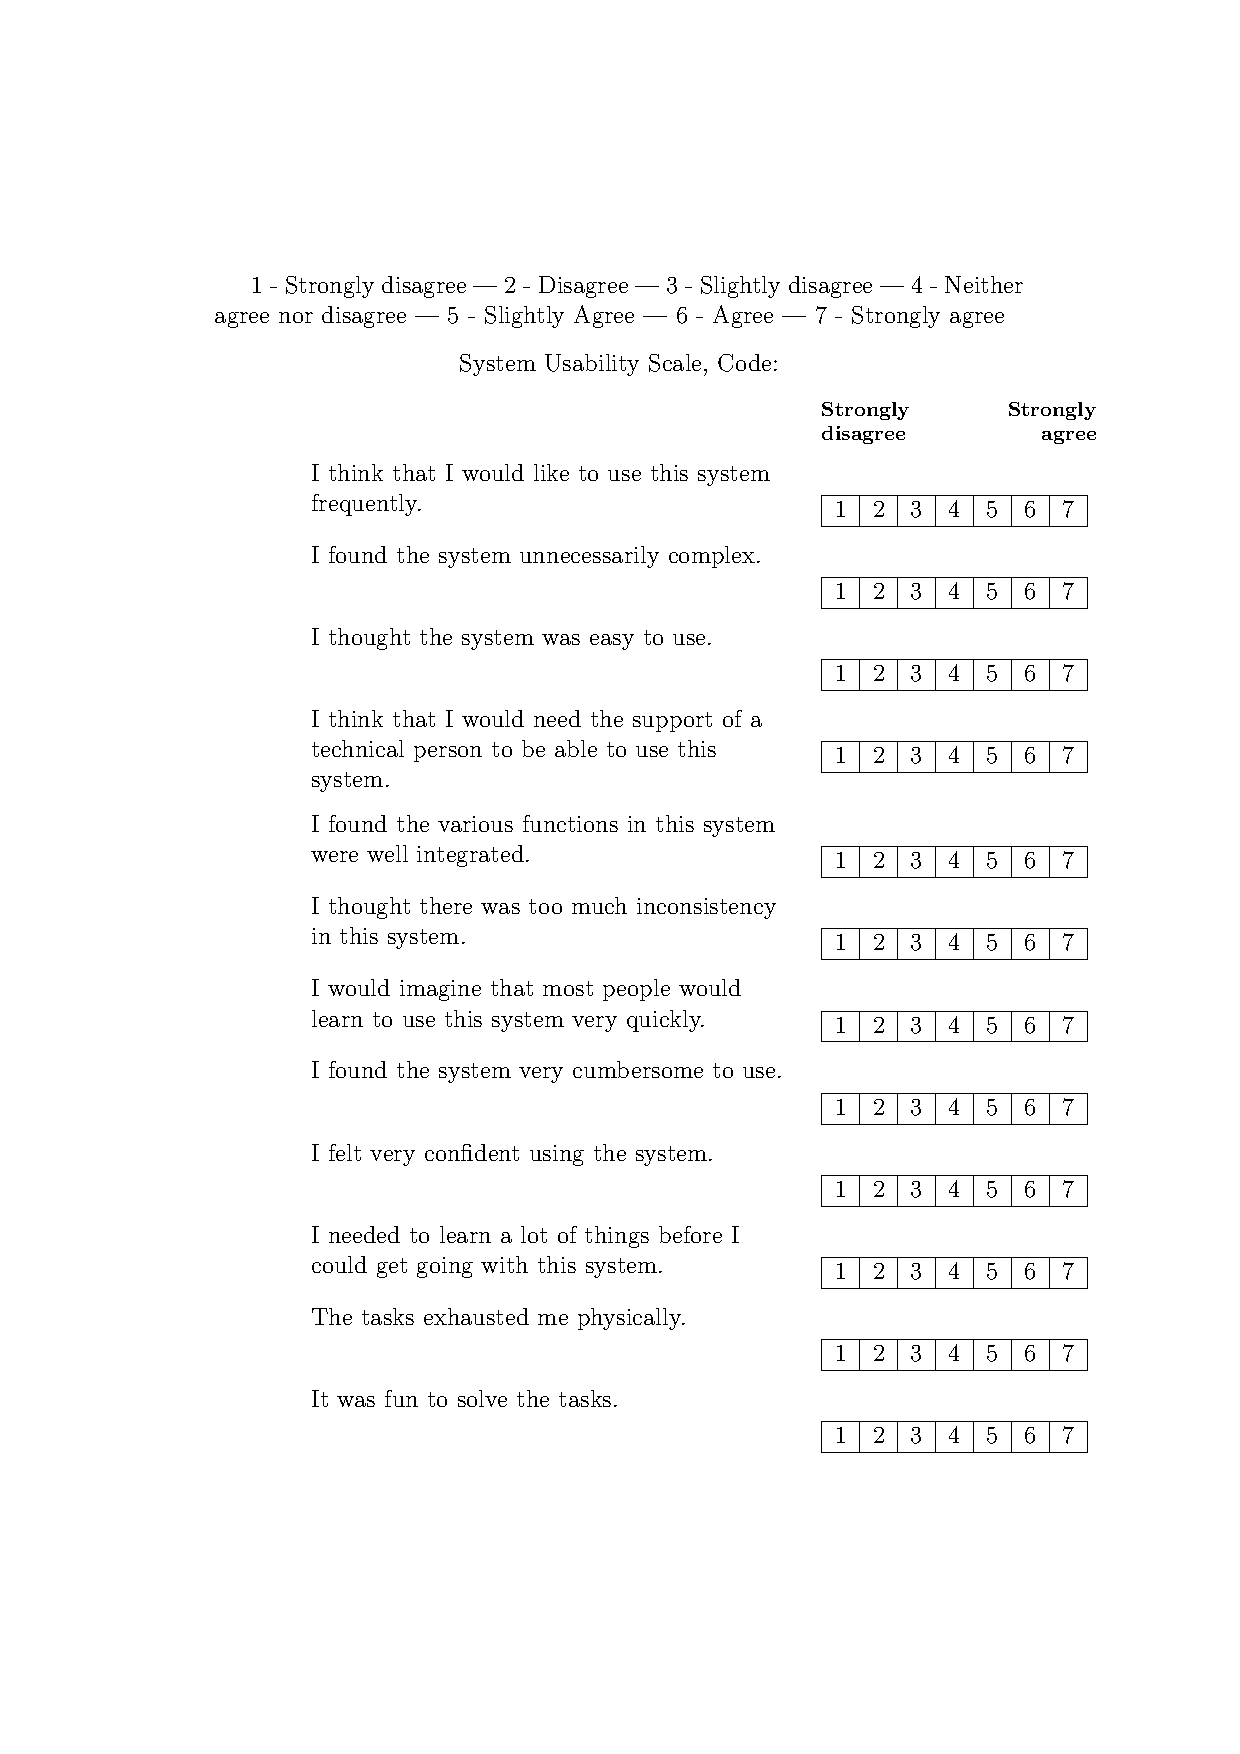
\includepdf[pages=-]{appendix/questionnaire.pdf}

\chapter{\label{appendix::B}B}
\begin{table}[h]
    \centering
    \begin{tabular}{llllll}
    \textbf{Participant} & \textbf{Age} & \textbf{Gender} & \textbf{Handed} & \textbf{Vision} & \textbf{Color Blindness} \\
    1             & 32           & m               & right           & normal          & false                     \\
    2             & 34           & m               & left            & normal          & false                     \\
    3             & 28           & m               & right           & normal          & false                     \\
    4             & 32           & m               & right           & corrected       & false                     \\
    5             & 34           & m               & right           & corrected       & false   
    \end{tabular}
    \begin{tabular}{lllll}
    \textbf{Participant} & \textbf{Q6} & \textbf{Q7} & \textbf{Q8} & \textbf{Q9} \\
        1             & b           & a           & c           & c           \\
        2             & b           & b           & b           & b           \\
        3             & b           & b           & b           & b           \\
        4             & b           & c           & c           & c           \\
        5             & c           & b           & c           & c          
    \end{tabular}
    \caption{Informations about the participants gathered in the pre-questionnaire.}
\end{table}